\documentclass[1p]{elsarticle_modified}
%\bibliographystyle{elsarticle-num}

%\usepackage[colorlinks]{hyperref}
%\usepackage{abbrmath_seonhwa} %\Abb, \Ascr, \Acal ,\Abf, \Afrak
\usepackage{amsfonts}
\usepackage{amssymb}
\usepackage{amsmath}
\usepackage{amsthm}
\usepackage{scalefnt}
\usepackage{amsbsy}
\usepackage{kotex}
\usepackage{caption}
\usepackage{subfig}
\usepackage{color}
\usepackage{graphicx}
\usepackage{xcolor} %% white, black, red, green, blue, cyan, magenta, yellow
\usepackage{float}
\usepackage{setspace}
\usepackage{hyperref}

\usepackage{tikz}
\usetikzlibrary{arrows}

\usepackage{multirow}
\usepackage{array} % fixed length table
\usepackage{hhline}

%%%%%%%%%%%%%%%%%%%%%
\makeatletter
\renewcommand*\env@matrix[1][\arraystretch]{%
	\edef\arraystretch{#1}%
	\hskip -\arraycolsep
	\let\@ifnextchar\new@ifnextchar
	\array{*\c@MaxMatrixCols c}}
\makeatother %https://tex.stackexchange.com/questions/14071/how-can-i-increase-the-line-spacing-in-a-matrix
%%%%%%%%%%%%%%%

\usepackage[normalem]{ulem}

\newcommand{\msout}[1]{\ifmmode\text{\sout{\ensuremath{#1}}}\else\sout{#1}\fi}
%SOURCE: \msout is \stkout macro in https://tex.stackexchange.com/questions/20609/strikeout-in-math-mode

\newcommand{\cancel}[1]{
	\ifmmode
	{\color{red}\msout{#1}}
	\else
	{\color{red}\sout{#1}}
	\fi
}

\newcommand{\add}[1]{
	{\color{blue}\uwave{#1}}
}

\newcommand{\replace}[2]{
	\ifmmode
	{\color{red}\msout{#1}}{\color{blue}\uwave{#2}}
	\else
	{\color{red}\sout{#1}}{\color{blue}\uwave{#2}}
	\fi
}

\newcommand{\Sol}{\mathcal{S}} %segment
\newcommand{\D}{D} %diagram
\newcommand{\A}{\mathcal{A}} %arc


%%%%%%%%%%%%%%%%%%%%%%%%%%%%%5 test

\def\sl{\operatorname{\textup{SL}}(2,\Cbb)}
\def\psl{\operatorname{\textup{PSL}}(2,\Cbb)}
\def\quan{\mkern 1mu \triangleright \mkern 1mu}

\theoremstyle{definition}
\newtheorem{thm}{Theorem}[section]
\newtheorem{prop}[thm]{Proposition}
\newtheorem{lem}[thm]{Lemma}
\newtheorem{ques}[thm]{Question}
\newtheorem{cor}[thm]{Corollary}
\newtheorem{defn}[thm]{Definition}
\newtheorem{exam}[thm]{Example}
\newtheorem{rmk}[thm]{Remark}
\newtheorem{alg}[thm]{Algorithm}

\newcommand{\I}{\sqrt{-1}}
\begin{document}

%\begin{frontmatter}
%
%\title{Boundary parabolic representations of knots up to 8 crossings}
%
%%% Group authors per affiliation:
%\author{Yunhi Cho} 
%\address{Department of Mathematics, University of Seoul, Seoul, Korea}
%\ead{yhcho@uos.ac.kr}
%
%
%\author{Seonhwa Kim} %\fnref{s_kim}}
%\address{Center for Geometry and Physics, Institute for Basic Science, Pohang, 37673, Korea}
%\ead{ryeona17@ibs.re.kr}
%
%\author{Hyuk Kim}
%\address{Department of Mathematical Sciences, Seoul National University, Seoul 08826, Korea}
%\ead{hyukkim@snu.ac.kr}
%
%\author{Seokbeom Yoon}
%\address{Department of Mathematical Sciences, Seoul National University, Seoul, 08826,  Korea}
%\ead{sbyoon15@snu.ac.kr}
%
%\begin{abstract}
%We find all boundary parabolic representation of knots up to 8 crossings.
%
%\end{abstract}
%\begin{keyword}
%    \MSC[2010] 57M25 
%\end{keyword}
%
%\end{frontmatter}

%\linenumbers
%\tableofcontents
%
\newcommand\colored[1]{\textcolor{white}{\rule[-0.35ex]{0.8em}{1.4ex}}\kern-0.8em\color{red} #1}%
%\newcommand\colored[1]{\textcolor{white}{ #1}\kern-2.17ex	\textcolor{white}{ #1}\kern-1.81ex	\textcolor{white}{ #1}\kern-2.15ex\color{red}#1	}

{\Large $\underline{12n_{0348}~(K12n_{0348})}$}

\setlength{\tabcolsep}{10pt}
\renewcommand{\arraystretch}{1.6}
\vspace{1cm}\begin{tabular}{m{100pt}>{\centering\arraybackslash}m{274pt}}
\multirow{5}{120pt}{
	\centering
	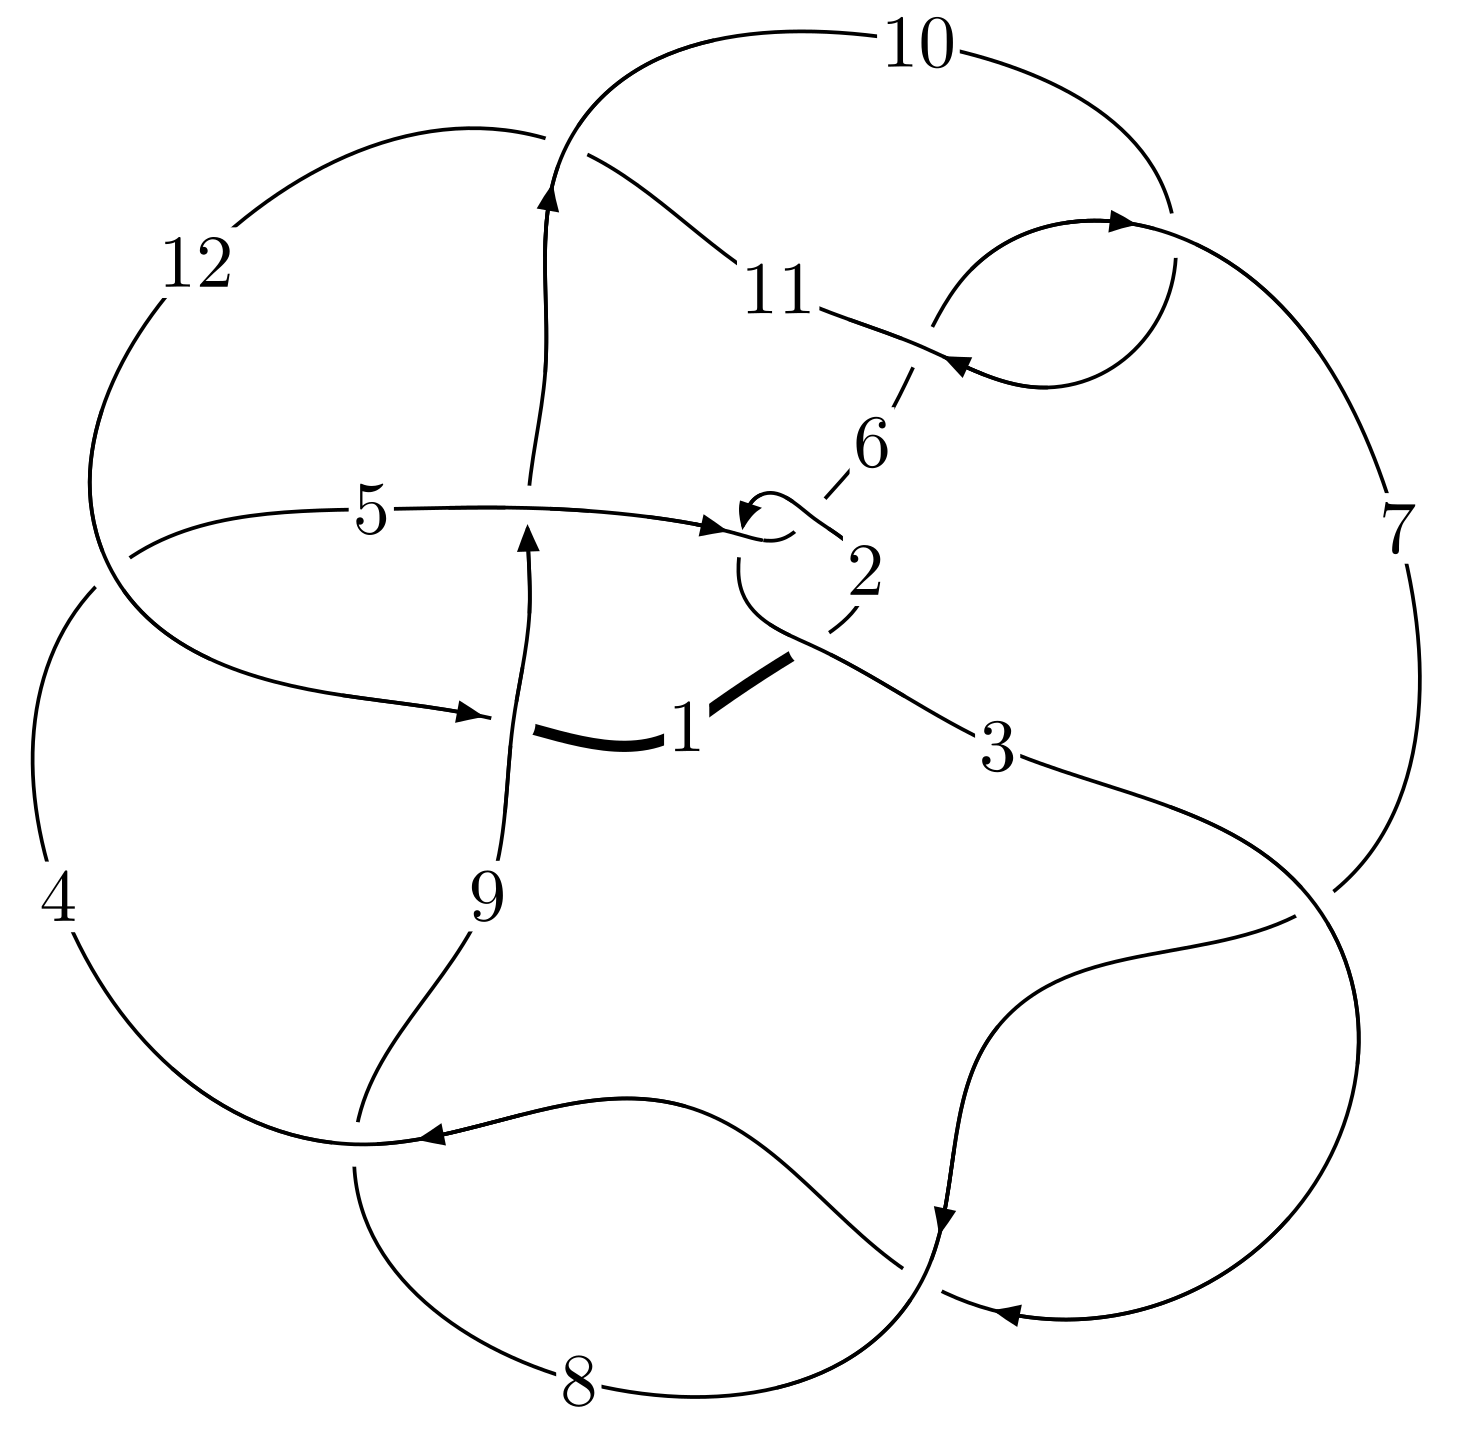
\includegraphics[width=112pt]{../../../GIT/diagram.site/Diagrams/png/2437_12n_0348.png}\\
\ \ \ A knot diagram\footnotemark}&
\allowdisplaybreaks
\textbf{Linearized knot diagam} \\
\cline{2-2}
 &
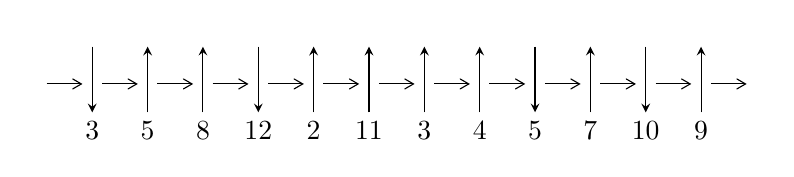
\begin{tikzpicture}[x=20pt, y=17pt]
	% nodes
	\node (C0) at (0, 0) {};
	\node (C1) at (1, 0) {};
	\node (C1U) at (1, +1) {};
	\node (C1D) at (1, -1) {3};

	\node (C2) at (2, 0) {};
	\node (C2U) at (2, +1) {};
	\node (C2D) at (2, -1) {5};

	\node (C3) at (3, 0) {};
	\node (C3U) at (3, +1) {};
	\node (C3D) at (3, -1) {8};

	\node (C4) at (4, 0) {};
	\node (C4U) at (4, +1) {};
	\node (C4D) at (4, -1) {12};

	\node (C5) at (5, 0) {};
	\node (C5U) at (5, +1) {};
	\node (C5D) at (5, -1) {2};

	\node (C6) at (6, 0) {};
	\node (C6U) at (6, +1) {};
	\node (C6D) at (6, -1) {11};

	\node (C7) at (7, 0) {};
	\node (C7U) at (7, +1) {};
	\node (C7D) at (7, -1) {3};

	\node (C8) at (8, 0) {};
	\node (C8U) at (8, +1) {};
	\node (C8D) at (8, -1) {4};

	\node (C9) at (9, 0) {};
	\node (C9U) at (9, +1) {};
	\node (C9D) at (9, -1) {5};

	\node (C10) at (10, 0) {};
	\node (C10U) at (10, +1) {};
	\node (C10D) at (10, -1) {7};

	\node (C11) at (11, 0) {};
	\node (C11U) at (11, +1) {};
	\node (C11D) at (11, -1) {10};

	\node (C12) at (12, 0) {};
	\node (C12U) at (12, +1) {};
	\node (C12D) at (12, -1) {9};
	\node (C13) at (13, 0) {};

	% arrows
	\draw[->,>={angle 60}]
	(C0) edge (C1) (C1) edge (C2) (C2) edge (C3) (C3) edge (C4) (C4) edge (C5) (C5) edge (C6) (C6) edge (C7) (C7) edge (C8) (C8) edge (C9) (C9) edge (C10) (C10) edge (C11) (C11) edge (C12) (C12) edge (C13) ;	\draw[->,>=stealth]
	(C1U) edge (C1D) (C2D) edge (C2U) (C3D) edge (C3U) (C4U) edge (C4D) (C5D) edge (C5U) (C6D) edge (C6U) (C7D) edge (C7U) (C8D) edge (C8U) (C9U) edge (C9D) (C10D) edge (C10U) (C11U) edge (C11D) (C12D) edge (C12U) ;
	\end{tikzpicture} \\
\hhline{~~} \\& 
\textbf{Solving Sequence} \\ \cline{2-2} 
 &
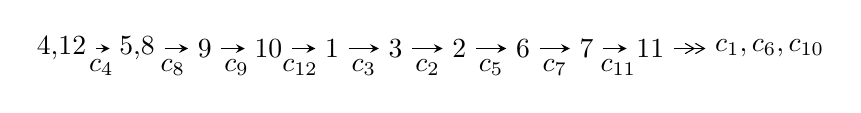
\begin{tikzpicture}[x=23pt, y=7pt]
	% node
	\node (A0) at (-1/8, 0) {4,12};
	\node (A1) at (17/16, 0) {5,8};
	\node (A2) at (17/8, 0) {9};
	\node (A3) at (25/8, 0) {10};
	\node (A4) at (33/8, 0) {1};
	\node (A5) at (41/8, 0) {3};
	\node (A6) at (49/8, 0) {2};
	\node (A7) at (57/8, 0) {6};
	\node (A8) at (65/8, 0) {7};
	\node (A9) at (73/8, 0) {11};
	\node (C1) at (1/2, -1) {$c_{4}$};
	\node (C2) at (13/8, -1) {$c_{8}$};
	\node (C3) at (21/8, -1) {$c_{9}$};
	\node (C4) at (29/8, -1) {$c_{12}$};
	\node (C5) at (37/8, -1) {$c_{3}$};
	\node (C6) at (45/8, -1) {$c_{2}$};
	\node (C7) at (53/8, -1) {$c_{5}$};
	\node (C8) at (61/8, -1) {$c_{7}$};
	\node (C9) at (69/8, -1) {$c_{11}$};
	\node (A10) at (11, 0) {$c_{1},c_{6},c_{10}$};

	% edge
	\draw[->,>=stealth]	
	(A0) edge (A1) (A1) edge (A2) (A2) edge (A3) (A3) edge (A4) (A4) edge (A5) (A5) edge (A6) (A6) edge (A7) (A7) edge (A8) (A8) edge (A9) ;
	\draw[->>,>={angle 60}]	
	(A9) edge (A10);
\end{tikzpicture} \\ 

\end{tabular} \\

\footnotetext{
The image of knot diagram is generated by the software ``\textbf{Draw programme}" developed by Andrew Bartholomew(\url{http://www.layer8.co.uk/maths/draw/index.htm\#Running-draw}), where we modified some parts for our purpose(\url{https://github.com/CATsTAILs/LinksPainter}).
}\phantom \\ \newline 
\centering \textbf{Ideals for irreducible components\footnotemark of $X_{\text{par}}$} 
 
\begin{align*}
I^u_{1}&=\langle 
2.60524\times10^{82} u^{54}+4.32163\times10^{82} u^{53}+\cdots+2.31107\times10^{83} b+9.23794\times10^{83},\\
\phantom{I^u_{1}}&\phantom{= \langle  }-5.24600\times10^{82} u^{54}-1.43004\times10^{83} u^{53}+\cdots+2.31107\times10^{83} a+3.49791\times10^{83},\\
\phantom{I^u_{1}}&\phantom{= \langle  }u^{55}+3 u^{54}+\cdots-12 u-11\rangle \\
I^u_{2}&=\langle 
u^{15}- u^{14}+\cdots+b+5,\;10 u^{15}-26 u^{14}+\cdots+a-13,\;u^{16}-2 u^{15}+\cdots+8 u^2+1\rangle \\
\\
\end{align*}
\raggedright * 2 irreducible components of $\dim_{\mathbb{C}}=0$, with total 71 representations.\\
\footnotetext{All coefficients of polynomials are rational numbers. But the coefficients are sometimes approximated in decimal forms when there is not enough margin.}
\newpage
\renewcommand{\arraystretch}{1}
\centering \section*{I. $I^u_{1}= \langle 2.61\times10^{82} u^{54}+4.32\times10^{82} u^{53}+\cdots+2.31\times10^{83} b+9.24\times10^{83},\;-5.25\times10^{82} u^{54}-1.43\times10^{83} u^{53}+\cdots+2.31\times10^{83} a+3.50\times10^{83},\;u^{55}+3 u^{54}+\cdots-12 u-11 \rangle$}
\flushleft \textbf{(i) Arc colorings}\\
\begin{tabular}{m{7pt} m{180pt} m{7pt} m{180pt} }
\flushright $a_{4}=$&$\begin{pmatrix}1\\0\end{pmatrix}$ \\
\flushright $a_{12}=$&$\begin{pmatrix}0\\u\end{pmatrix}$ \\
\flushright $a_{5}=$&$\begin{pmatrix}1\\u^2\end{pmatrix}$ \\
\flushright $a_{8}=$&$\begin{pmatrix}0.226994 u^{54}+0.618778 u^{53}+\cdots-10.4791 u-1.51354\\-0.112728 u^{54}-0.186996 u^{53}+\cdots-4.08158 u-3.99725\end{pmatrix}$ \\
\flushright $a_{9}=$&$\begin{pmatrix}0.114266 u^{54}+0.431782 u^{53}+\cdots-14.5607 u-5.51080\\-0.112728 u^{54}-0.186996 u^{53}+\cdots-4.08158 u-3.99725\end{pmatrix}$ \\
\flushright $a_{10}=$&$\begin{pmatrix}0.107387 u^{54}+0.305810 u^{53}+\cdots-8.15437 u-0.534709\\-0.0799915 u^{54}-0.0948860 u^{53}+\cdots-5.42127 u-5.15595\end{pmatrix}$ \\
\flushright $a_{1}=$&$\begin{pmatrix}0.908704 u^{54}+3.08911 u^{53}+\cdots-23.8651 u-16.2385\\-0.447095 u^{54}-1.15334 u^{53}+\cdots+7.94778 u-2.70823\end{pmatrix}$ \\
\flushright $a_{3}=$&$\begin{pmatrix}-0.172479 u^{54}-1.13662 u^{53}+\cdots+24.4494 u+14.6350\\-0.0737233 u^{54}-0.0490777 u^{53}+\cdots+2.74375 u-3.73277\end{pmatrix}$ \\
\flushright $a_{2}=$&$\begin{pmatrix}0.0660274 u^{54}-0.351978 u^{53}+\cdots+12.3782 u+11.5567\\-0.207205 u^{54}-0.434267 u^{53}+\cdots+6.19685 u-2.97237\end{pmatrix}$ \\
\flushright $a_{6}=$&$\begin{pmatrix}0.0217548 u^{54}-0.00585046 u^{53}+\cdots-3.61926 u-1.19908\\0.340641 u^{54}+0.992765 u^{53}+\cdots-11.1110 u+1.49013\end{pmatrix}$ \\
\flushright $a_{7}=$&$\begin{pmatrix}0.281862 u^{54}+1.12478 u^{53}+\cdots-14.1050 u-9.98072\\-0.0168458 u^{54}-0.208276 u^{53}+\cdots+6.42777 u+1.43253\end{pmatrix}$ \\
\flushright $a_{11}=$&$\begin{pmatrix}0.520294 u^{54}+1.83552 u^{53}+\cdots-15.1557 u-6.44576\\-0.335273 u^{54}-1.03983 u^{53}+\cdots+8.71346 u-0.0705450\end{pmatrix}$\\&\end{tabular}
\flushleft \textbf{(ii) Obstruction class $= -1$}\\~\\
\flushleft \textbf{(iii) Cusp Shapes $= -0.313768 u^{54}-0.790410 u^{53}+\cdots+2.10169 u-8.23967$}\\~\\
\newpage\renewcommand{\arraystretch}{1}
\flushleft \textbf{(iv) u-Polynomials at the component}\newline \\
\begin{tabular}{m{50pt}|m{274pt}}
Crossings & \hspace{64pt}u-Polynomials at each crossing \\
\hline $$\begin{aligned}c_{1}\end{aligned}$$&$\begin{aligned}
&u^{55}+63 u^{54}+\cdots-20918 u-169
\end{aligned}$\\
\hline $$\begin{aligned}c_{2},c_{5}\end{aligned}$$&$\begin{aligned}
&u^{55}+u^{54}+\cdots+86 u-13
\end{aligned}$\\
\hline $$\begin{aligned}c_{3},c_{7},c_{8}\end{aligned}$$&$\begin{aligned}
&u^{55}+u^{54}+\cdots+22 u^2-23
\end{aligned}$\\
\hline $$\begin{aligned}c_{4}\end{aligned}$$&$\begin{aligned}
&u^{55}+3 u^{54}+\cdots-12 u-11
\end{aligned}$\\
\hline $$\begin{aligned}c_{6},c_{10}\end{aligned}$$&$\begin{aligned}
&u^{55}-3 u^{54}+\cdots+84 u-17
\end{aligned}$\\
\hline $$\begin{aligned}c_{9}\end{aligned}$$&$\begin{aligned}
&u^{55}- u^{54}+\cdots-325045 u-237989
\end{aligned}$\\
\hline $$\begin{aligned}c_{11}\end{aligned}$$&$\begin{aligned}
&u^{55}+37 u^{54}+\cdots-1784 u-289
\end{aligned}$\\
\hline $$\begin{aligned}c_{12}\end{aligned}$$&$\begin{aligned}
&u^{55}+11 u^{54}+\cdots+89882 u+16337
\end{aligned}$\\
\hline
\end{tabular}\\~\\
\newpage\renewcommand{\arraystretch}{1}
\flushleft \textbf{(v) Riley Polynomials at the component}\newline \\
\begin{tabular}{m{50pt}|m{274pt}}
Crossings & \hspace{64pt}Riley Polynomials at each crossing \\
\hline $$\begin{aligned}c_{1}\end{aligned}$$&$\begin{aligned}
&y^{55}-137 y^{54}+\cdots+108847246 y-28561
\end{aligned}$\\
\hline $$\begin{aligned}c_{2},c_{5}\end{aligned}$$&$\begin{aligned}
&y^{55}+63 y^{54}+\cdots-20918 y-169
\end{aligned}$\\
\hline $$\begin{aligned}c_{3},c_{7},c_{8}\end{aligned}$$&$\begin{aligned}
&y^{55}-43 y^{54}+\cdots+1012 y-529
\end{aligned}$\\
\hline $$\begin{aligned}c_{4}\end{aligned}$$&$\begin{aligned}
&y^{55}+21 y^{54}+\cdots-4740 y-121
\end{aligned}$\\
\hline $$\begin{aligned}c_{6},c_{10}\end{aligned}$$&$\begin{aligned}
&y^{55}+37 y^{54}+\cdots-1784 y-289
\end{aligned}$\\
\hline $$\begin{aligned}c_{9}\end{aligned}$$&$\begin{aligned}
&y^{55}-23 y^{54}+\cdots-63034731065 y-56638764121
\end{aligned}$\\
\hline $$\begin{aligned}c_{11}\end{aligned}$$&$\begin{aligned}
&y^{55}-27 y^{54}+\cdots-78420 y-83521
\end{aligned}$\\
\hline $$\begin{aligned}c_{12}\end{aligned}$$&$\begin{aligned}
&y^{55}-3 y^{54}+\cdots+4960988170 y-266897569
\end{aligned}$\\
\hline
\end{tabular}\\~\\
\newpage\flushleft \textbf{(vi) Complex Volumes and Cusp Shapes}
$$\begin{array}{c|c|c}  
\text{Solutions to }I^u_{1}& \I (\text{vol} + \sqrt{-1}CS) & \text{Cusp shape}\\
 \hline 
\begin{aligned}
u &= -0.815485 + 0.609992 I \\
a &= \phantom{-}0.716376 - 0.340161 I \\
b &= -1.240990 + 0.607346 I\end{aligned}
 & -3.46247 - 2.90307 I & \phantom{-}4.19084 + 1.32778 I \\ \hline\begin{aligned}
u &= -0.815485 - 0.609992 I \\
a &= \phantom{-}0.716376 + 0.340161 I \\
b &= -1.240990 - 0.607346 I\end{aligned}
 & -3.46247 + 2.90307 I & \phantom{-}4.19084 - 1.32778 I \\ \hline\begin{aligned}
u &= -0.766697 + 0.587191 I \\
a &= \phantom{-}0.121340 - 0.656968 I \\
b &= -0.288763 - 0.617191 I\end{aligned}
 & -3.36899 + 1.08421 I & -1.34816 - 2.39352 I \\ \hline\begin{aligned}
u &= -0.766697 - 0.587191 I \\
a &= \phantom{-}0.121340 + 0.656968 I \\
b &= -0.288763 + 0.617191 I\end{aligned}
 & -3.36899 - 1.08421 I & -1.34816 + 2.39352 I \\ \hline\begin{aligned}
u &= -0.342407 + 0.888408 I \\
a &= -0.352056 + 0.222676 I \\
b &= \phantom{-}0.093000 + 0.425608 I\end{aligned}
 & \phantom{-}0.55048 + 1.48371 I & \phantom{-}4.97976 - 5.81830 I \\ \hline\begin{aligned}
u &= -0.342407 - 0.888408 I \\
a &= -0.352056 - 0.222676 I \\
b &= \phantom{-}0.093000 - 0.425608 I\end{aligned}
 & \phantom{-}0.55048 - 1.48371 I & \phantom{-}4.97976 + 5.81830 I \\ \hline\begin{aligned}
u &= -0.181810 + 1.053110 I \\
a &= -0.138751 + 0.733731 I \\
b &= \phantom{-}0.759862 + 0.688944 I\end{aligned}
 & -3.21509 + 2.62066 I & \phantom{-}1.87813 - 3.80550 I \\ \hline\begin{aligned}
u &= -0.181810 - 1.053110 I \\
a &= -0.138751 - 0.733731 I \\
b &= \phantom{-}0.759862 - 0.688944 I\end{aligned}
 & -3.21509 - 2.62066 I & \phantom{-}1.87813 + 3.80550 I \\ \hline\begin{aligned}
u &= -0.722892 + 0.803711 I \\
a &= \phantom{-}2.14118 - 1.56678 I \\
b &= -1.38166 - 0.45730 I\end{aligned}
 & -7.22887 + 2.83374 I & \phantom{-}2.38389 - 3.49922 I \\ \hline\begin{aligned}
u &= -0.722892 - 0.803711 I \\
a &= \phantom{-}2.14118 + 1.56678 I \\
b &= -1.38166 + 0.45730 I\end{aligned}
 & -7.22887 - 2.83374 I & \phantom{-}2.38389 + 3.49922 I\\
 \hline 
 \end{array}$$\newpage$$\begin{array}{c|c|c}  
\text{Solutions to }I^u_{1}& \I (\text{vol} + \sqrt{-1}CS) & \text{Cusp shape}\\
 \hline 
\begin{aligned}
u &= \phantom{-}0.173002 + 0.887529 I \\
a &= \phantom{-}2.29349 + 0.99676 I \\
b &= -1.53634 + 0.17332 I\end{aligned}
 & \phantom{-}7.27746 - 3.45379 I & \phantom{-}10.27416 + 1.32847 I \\ \hline\begin{aligned}
u &= \phantom{-}0.173002 - 0.887529 I \\
a &= \phantom{-}2.29349 - 0.99676 I \\
b &= -1.53634 - 0.17332 I\end{aligned}
 & \phantom{-}7.27746 + 3.45379 I & \phantom{-}10.27416 - 1.32847 I \\ \hline\begin{aligned}
u &= \phantom{-}0.628360 + 0.597283 I \\
a &= \phantom{-}1.092470 - 0.206282 I \\
b &= -0.537582 - 0.337146 I\end{aligned}
 & -0.59371 - 3.25938 I & \phantom{-}2.97394 - 0.66796 I \\ \hline\begin{aligned}
u &= \phantom{-}0.628360 - 0.597283 I \\
a &= \phantom{-}1.092470 + 0.206282 I \\
b &= -0.537582 + 0.337146 I\end{aligned}
 & -0.59371 + 3.25938 I & \phantom{-}2.97394 + 0.66796 I \\ \hline\begin{aligned}
u &= -0.711127 + 0.948848 I \\
a &= -0.966349 + 0.247086 I \\
b &= \phantom{-}1.34857 - 0.64792 I\end{aligned}
 & -6.77729 + 2.66101 I & \phantom{-0.000000 } 0 \\ \hline\begin{aligned}
u &= -0.711127 - 0.948848 I \\
a &= -0.966349 - 0.247086 I \\
b &= \phantom{-}1.34857 + 0.64792 I\end{aligned}
 & -6.77729 - 2.66101 I & \phantom{-0.000000 } 0 \\ \hline\begin{aligned}
u &= \phantom{-}0.800334 + 0.884723 I \\
a &= \phantom{-}0.677563 - 0.092095 I \\
b &= -0.119062 + 1.076690 I\end{aligned}
 & -6.90102 - 2.99599 I & \phantom{-0.000000 } 0 \\ \hline\begin{aligned}
u &= \phantom{-}0.800334 - 0.884723 I \\
a &= \phantom{-}0.677563 + 0.092095 I \\
b &= -0.119062 - 1.076690 I\end{aligned}
 & -6.90102 + 2.99599 I & \phantom{-0.000000 } 0 \\ \hline\begin{aligned}
u &= -0.598983 + 1.067040 I \\
a &= \phantom{-}0.455882 - 0.093492 I \\
b &= \phantom{-}0.309654 - 0.497235 I\end{aligned}
 & -1.80177 + 4.16956 I & \phantom{-0.000000 } 0 \\ \hline\begin{aligned}
u &= -0.598983 - 1.067040 I \\
a &= \phantom{-}0.455882 + 0.093492 I \\
b &= \phantom{-}0.309654 + 0.497235 I\end{aligned}
 & -1.80177 - 4.16956 I & \phantom{-0.000000 } 0\\
 \hline 
 \end{array}$$\newpage$$\begin{array}{c|c|c}  
\text{Solutions to }I^u_{1}& \I (\text{vol} + \sqrt{-1}CS) & \text{Cusp shape}\\
 \hline 
\begin{aligned}
u &= \phantom{-}0.992759 + 0.740017 I \\
a &= -0.766608 - 0.114418 I \\
b &= \phantom{-}0.059829 - 0.980635 I\end{aligned}
 & -11.75940 + 2.31711 I & \phantom{-0.000000 } 0 \\ \hline\begin{aligned}
u &= \phantom{-}0.992759 - 0.740017 I \\
a &= -0.766608 + 0.114418 I \\
b &= \phantom{-}0.059829 + 0.980635 I\end{aligned}
 & -11.75940 - 2.31711 I & \phantom{-0.000000 } 0 \\ \hline\begin{aligned}
u &= \phantom{-}0.682830 + 0.316170 I \\
a &= \phantom{-}0.666716 - 0.682016 I \\
b &= -0.911518 - 0.401923 I\end{aligned}
 & -1.67294 + 2.77507 I & \phantom{-}2.05247 - 3.78121 I \\ \hline\begin{aligned}
u &= \phantom{-}0.682830 - 0.316170 I \\
a &= \phantom{-}0.666716 + 0.682016 I \\
b &= -0.911518 + 0.401923 I\end{aligned}
 & -1.67294 - 2.77507 I & \phantom{-}2.05247 + 3.78121 I \\ \hline\begin{aligned}
u &= -0.648251 + 1.072510 I \\
a &= -0.698611 + 0.921968 I \\
b &= \phantom{-}0.946204 + 0.085319 I\end{aligned}
 & \phantom{-}1.85295 + 1.10015 I & \phantom{-0.000000 } 0 \\ \hline\begin{aligned}
u &= -0.648251 - 1.072510 I \\
a &= -0.698611 - 0.921968 I \\
b &= \phantom{-}0.946204 - 0.085319 I\end{aligned}
 & \phantom{-}1.85295 - 1.10015 I & \phantom{-0.000000 } 0 \\ \hline\begin{aligned}
u &= \phantom{-}0.577460 + 1.116900 I \\
a &= -1.83686 - 1.43049 I \\
b &= \phantom{-}1.113190 - 0.366716 I\end{aligned}
 & \phantom{-}0.58204 - 7.69168 I & \phantom{-0.000000 } 0 \\ \hline\begin{aligned}
u &= \phantom{-}0.577460 - 1.116900 I \\
a &= -1.83686 + 1.43049 I \\
b &= \phantom{-}1.113190 + 0.366716 I\end{aligned}
 & \phantom{-}0.58204 + 7.69168 I & \phantom{-0.000000 } 0 \\ \hline\begin{aligned}
u &= \phantom{-}0.461578 + 1.175220 I \\
a &= \phantom{-}1.85272 + 0.82840 I \\
b &= -1.234160 + 0.257600 I\end{aligned}
 & \phantom{-}4.47795 - 4.19285 I & \phantom{-0.000000 } 0 \\ \hline\begin{aligned}
u &= \phantom{-}0.461578 - 1.175220 I \\
a &= \phantom{-}1.85272 - 0.82840 I \\
b &= -1.234160 - 0.257600 I\end{aligned}
 & \phantom{-}4.47795 + 4.19285 I & \phantom{-0.000000 } 0\\
 \hline 
 \end{array}$$\newpage$$\begin{array}{c|c|c}  
\text{Solutions to }I^u_{1}& \I (\text{vol} + \sqrt{-1}CS) & \text{Cusp shape}\\
 \hline 
\begin{aligned}
u &= -0.264238 + 0.685778 I \\
a &= \phantom{-}0.53501 - 4.66877 I \\
b &= -0.937038 + 0.123287 I\end{aligned}
 & -4.80330 - 0.56532 I & \phantom{-}4.34221 - 3.19087 I \\ \hline\begin{aligned}
u &= -0.264238 - 0.685778 I \\
a &= \phantom{-}0.53501 + 4.66877 I \\
b &= -0.937038 - 0.123287 I\end{aligned}
 & -4.80330 + 0.56532 I & \phantom{-}4.34221 + 3.19087 I \\ \hline\begin{aligned}
u &= -0.712473 + 1.066430 I \\
a &= -1.88688 + 1.00057 I \\
b &= \phantom{-}1.41881 + 0.51710 I\end{aligned}
 & -2.09404 + 8.67779 I & \phantom{-0.000000 } 0 \\ \hline\begin{aligned}
u &= -0.712473 - 1.066430 I \\
a &= -1.88688 - 1.00057 I \\
b &= \phantom{-}1.41881 - 0.51710 I\end{aligned}
 & -2.09404 - 8.67779 I & \phantom{-0.000000 } 0 \\ \hline\begin{aligned}
u &= -0.004077 + 0.715907 I \\
a &= -3.38106 - 1.04947 I \\
b &= \phantom{-}1.53871 + 0.03923 I\end{aligned}
 & \phantom{-}6.53124 + 2.75926 I & \phantom{-}7.77095 - 4.45417 I \\ \hline\begin{aligned}
u &= -0.004077 - 0.715907 I \\
a &= -3.38106 + 1.04947 I \\
b &= \phantom{-}1.53871 - 0.03923 I\end{aligned}
 & \phantom{-}6.53124 - 2.75926 I & \phantom{-}7.77095 + 4.45417 I \\ \hline\begin{aligned}
u &= \phantom{-}0.119783 + 0.703838 I \\
a &= -0.805794 + 0.305998 I \\
b &= \phantom{-}0.362409 + 0.453693 I\end{aligned}
 & \phantom{-}1.003320 + 0.902305 I & \phantom{-}8.30926 - 5.19000 I \\ \hline\begin{aligned}
u &= \phantom{-}0.119783 - 0.703838 I \\
a &= -0.805794 - 0.305998 I \\
b &= \phantom{-}0.362409 - 0.453693 I\end{aligned}
 & \phantom{-}1.003320 - 0.902305 I & \phantom{-}8.30926 + 5.19000 I \\ \hline\begin{aligned}
u &= \phantom{-}0.995644 + 0.888830 I \\
a &= -1.031330 - 0.818819 I \\
b &= \phantom{-}1.356040 - 0.197721 I\end{aligned}
 & \phantom{-}1.77258 - 3.90284 I & \phantom{-0.000000 } 0 \\ \hline\begin{aligned}
u &= \phantom{-}0.995644 - 0.888830 I \\
a &= -1.031330 + 0.818819 I \\
b &= \phantom{-}1.356040 + 0.197721 I\end{aligned}
 & \phantom{-}1.77258 + 3.90284 I & \phantom{-0.000000 } 0\\
 \hline 
 \end{array}$$\newpage$$\begin{array}{c|c|c}  
\text{Solutions to }I^u_{1}& \I (\text{vol} + \sqrt{-1}CS) & \text{Cusp shape}\\
 \hline 
\begin{aligned}
u &= \phantom{-}0.126954 + 1.333810 I \\
a &= -1.95011 + 0.22052 I \\
b &= \phantom{-}1.128790 - 0.066319 I\end{aligned}
 & \phantom{-}3.06772 - 0.82361 I & \phantom{-0.000000 } 0 \\ \hline\begin{aligned}
u &= \phantom{-}0.126954 - 1.333810 I \\
a &= -1.95011 - 0.22052 I \\
b &= \phantom{-}1.128790 + 0.066319 I\end{aligned}
 & \phantom{-}3.06772 + 0.82361 I & \phantom{-0.000000 } 0 \\ \hline\begin{aligned}
u &= \phantom{-}0.813384 + 1.075410 I \\
a &= -0.501571 + 0.076047 I \\
b &= \phantom{-}0.070094 - 1.130120 I\end{aligned}
 & -10.66830 - 8.91439 I & \phantom{-0.000000 } 0 \\ \hline\begin{aligned}
u &= \phantom{-}0.813384 - 1.075410 I \\
a &= -0.501571 - 0.076047 I \\
b &= \phantom{-}0.070094 + 1.130120 I\end{aligned}
 & -10.66830 + 8.91439 I & \phantom{-0.000000 } 0 \\ \hline\begin{aligned}
u &= \phantom{-}0.650155\phantom{ +0.000000I} \\
a &= -0.555963\phantom{ +0.000000I} \\
b &= \phantom{-}0.901498\phantom{ +0.000000I}\end{aligned}
 & \phantom{-}1.30158\phantom{ +0.000000I} & \phantom{-}8.19850\phantom{ +0.000000I} \\ \hline\begin{aligned}
u &= -1.222360 + 0.639856 I \\
a &= -0.680782 + 0.122900 I \\
b &= \phantom{-}1.288840 - 0.499125 I\end{aligned}
 & -7.94459 - 7.58411 I & \phantom{-0.000000 } 0 \\ \hline\begin{aligned}
u &= -1.222360 - 0.639856 I \\
a &= -0.680782 - 0.122900 I \\
b &= \phantom{-}1.288840 + 0.499125 I\end{aligned}
 & -7.94459 + 7.58411 I & \phantom{-0.000000 } 0 \\ \hline\begin{aligned}
u &= -1.035520 + 0.922159 I \\
a &= \phantom{-}0.550770 - 0.481659 I \\
b &= -0.990991 - 0.201391 I\end{aligned}
 & \phantom{-}0.50650 + 5.61395 I & \phantom{-0.000000 } 0 \\ \hline\begin{aligned}
u &= -1.035520 - 0.922159 I \\
a &= \phantom{-}0.550770 + 0.481659 I \\
b &= -0.990991 + 0.201391 I\end{aligned}
 & \phantom{-}0.50650 - 5.61395 I & \phantom{-0.000000 } 0 \\ \hline\begin{aligned}
u &= -0.82989 + 1.20266 I \\
a &= \phantom{-}1.60979 - 0.92855 I \\
b &= -1.40604 - 0.54304 I\end{aligned}
 & -6.0591 + 14.8324 I & \phantom{-0.000000 } 0\\
 \hline 
 \end{array}$$\newpage$$\begin{array}{c|c|c}  
\text{Solutions to }I^u_{1}& \I (\text{vol} + \sqrt{-1}CS) & \text{Cusp shape}\\
 \hline 
\begin{aligned}
u &= -0.82989 - 1.20266 I \\
a &= \phantom{-}1.60979 + 0.92855 I \\
b &= -1.40604 + 0.54304 I\end{aligned}
 & -6.0591 - 14.8324 I & \phantom{-0.000000 } 0 \\ \hline\begin{aligned}
u &= \phantom{-}0.69303 + 1.48402 I \\
a &= \phantom{-}1.37520 + 0.37724 I \\
b &= -1.330370 + 0.097750 I\end{aligned}
 & \phantom{-}3.52220 - 3.74412 I & \phantom{-0.000000 } 0 \\ \hline\begin{aligned}
u &= \phantom{-}0.69303 - 1.48402 I \\
a &= \phantom{-}1.37520 - 0.37724 I \\
b &= -1.330370 - 0.097750 I\end{aligned}
 & \phantom{-}3.52220 + 3.74412 I & \phantom{-0.000000 } 0 \\ \hline\begin{aligned}
u &= -0.033996 + 0.282179 I \\
a &= -0.63193 - 1.74588 I \\
b &= -0.830222 - 0.601183 I\end{aligned}
 & -1.96989 + 2.37563 I & -2.00410 - 0.86695 I \\ \hline\begin{aligned}
u &= -0.033996 - 0.282179 I \\
a &= -0.63193 + 1.74588 I \\
b &= -0.830222 + 0.601183 I\end{aligned}
 & -1.96989 - 2.37563 I & -2.00410 + 0.86695 I\\
 \hline 
 \end{array}$$\newpage\newpage\renewcommand{\arraystretch}{1}
\centering \section*{II. $I^u_{2}= \langle u^{15}- u^{14}+\cdots+b+5,\;10 u^{15}-26 u^{14}+\cdots+a-13,\;u^{16}-2 u^{15}+\cdots+8 u^2+1 \rangle$}
\flushleft \textbf{(i) Arc colorings}\\
\begin{tabular}{m{7pt} m{180pt} m{7pt} m{180pt} }
\flushright $a_{4}=$&$\begin{pmatrix}1\\0\end{pmatrix}$ \\
\flushright $a_{12}=$&$\begin{pmatrix}0\\u\end{pmatrix}$ \\
\flushright $a_{5}=$&$\begin{pmatrix}1\\u^2\end{pmatrix}$ \\
\flushright $a_{8}=$&$\begin{pmatrix}-10 u^{15}+26 u^{14}+\cdots-32 u+13\\- u^{15}+u^{14}+\cdots-6 u-5\end{pmatrix}$ \\
\flushright $a_{9}=$&$\begin{pmatrix}-11 u^{15}+27 u^{14}+\cdots-38 u+8\\- u^{15}+u^{14}+\cdots-6 u-5\end{pmatrix}$ \\
\flushright $a_{10}=$&$\begin{pmatrix}-6 u^{15}+16 u^{14}+\cdots-21 u+8\\-2 u^{15}+4 u^{14}+\cdots-11 u-4\end{pmatrix}$ \\
\flushright $a_{1}=$&$\begin{pmatrix}-26 u^{15}+57 u^{14}+\cdots-103 u+12\\- u^{15}+u^{14}+\cdots-5 u-7\end{pmatrix}$ \\
\flushright $a_{3}=$&$\begin{pmatrix}6 u^{15}-13 u^{14}+\cdots+31 u-6\\u^{15}-2 u^{14}+\cdots+2 u+1\end{pmatrix}$ \\
\flushright $a_{2}=$&$\begin{pmatrix}5 u^{15}-11 u^{14}+\cdots+23 u-6\\u^{15}-2 u^{14}+\cdots+3 u+1\end{pmatrix}$ \\
\flushright $a_{6}=$&$\begin{pmatrix}6 u^{15}-7 u^{14}+\cdots+20 u+24\\- u^{15}+3 u^{14}+\cdots-8 u+3\end{pmatrix}$ \\
\flushright $a_{7}=$&$\begin{pmatrix}-2 u^{15}-8 u^{13}+\cdots-10 u-10\\-3 u^{15}+6 u^{14}+\cdots+2 u-1\end{pmatrix}$ \\
\flushright $a_{11}=$&$\begin{pmatrix}-13 u^{15}+30 u^{14}+\cdots-46 u+14\\-2 u^{15}+5 u^{14}+\cdots-11 u-4\end{pmatrix}$\\&\end{tabular}
\flushleft \textbf{(ii) Obstruction class $= 1$}\\~\\
\flushleft \textbf{(iii) Cusp Shapes $= -13 u^{15}+19 u^{14}-69 u^{13}+42 u^{12}-161 u^{11}+50 u^{10}-278 u^9-24 u^8-320 u^7-121 u^6-269 u^5-156 u^4-127 u^3-89 u^2-34 u-13$}\\~\\
\newpage\renewcommand{\arraystretch}{1}
\flushleft \textbf{(iv) u-Polynomials at the component}\newline \\
\begin{tabular}{m{50pt}|m{274pt}}
Crossings & \hspace{64pt}u-Polynomials at each crossing \\
\hline $$\begin{aligned}c_{1}\end{aligned}$$&$\begin{aligned}
&u^{16}-16 u^{15}+\cdots-10 u+1
\end{aligned}$\\
\hline $$\begin{aligned}c_{2}\end{aligned}$$&$\begin{aligned}
&u^{16}+8 u^{14}+\cdots-2 u+1
\end{aligned}$\\
\hline $$\begin{aligned}c_{3}\end{aligned}$$&$\begin{aligned}
&u^{16}-9 u^{14}+\cdots-2 u+1
\end{aligned}$\\
\hline $$\begin{aligned}c_{4}\end{aligned}$$&$\begin{aligned}
&u^{16}-2 u^{15}+\cdots+8 u^2+1
\end{aligned}$\\
\hline $$\begin{aligned}c_{5}\end{aligned}$$&$\begin{aligned}
&u^{16}+8 u^{14}+\cdots+2 u+1
\end{aligned}$\\
\hline $$\begin{aligned}c_{6}\end{aligned}$$&$\begin{aligned}
&u^{16}-2 u^{15}+\cdots+6 u^2+1
\end{aligned}$\\
\hline $$\begin{aligned}c_{7},c_{8}\end{aligned}$$&$\begin{aligned}
&u^{16}-9 u^{14}+\cdots+2 u+1
\end{aligned}$\\
\hline $$\begin{aligned}c_{9}\end{aligned}$$&$\begin{aligned}
&u^{16}+5 u^{14}+\cdots- u+1
\end{aligned}$\\
\hline $$\begin{aligned}c_{10}\end{aligned}$$&$\begin{aligned}
&u^{16}+2 u^{15}+\cdots+6 u^2+1
\end{aligned}$\\
\hline $$\begin{aligned}c_{11}\end{aligned}$$&$\begin{aligned}
&u^{16}+10 u^{15}+\cdots+12 u+1
\end{aligned}$\\
\hline $$\begin{aligned}c_{12}\end{aligned}$$&$\begin{aligned}
&u^{16}+4 u^{15}+\cdots-4 u+1
\end{aligned}$\\
\hline
\end{tabular}\\~\\
\newpage\renewcommand{\arraystretch}{1}
\flushleft \textbf{(v) Riley Polynomials at the component}\newline \\
\begin{tabular}{m{50pt}|m{274pt}}
Crossings & \hspace{64pt}Riley Polynomials at each crossing \\
\hline $$\begin{aligned}c_{1}\end{aligned}$$&$\begin{aligned}
&y^{16}-28 y^{15}+\cdots+14 y+1
\end{aligned}$\\
\hline $$\begin{aligned}c_{2},c_{5}\end{aligned}$$&$\begin{aligned}
&y^{16}+16 y^{15}+\cdots+10 y+1
\end{aligned}$\\
\hline $$\begin{aligned}c_{3},c_{7},c_{8}\end{aligned}$$&$\begin{aligned}
&y^{16}-18 y^{15}+\cdots-8 y+1
\end{aligned}$\\
\hline $$\begin{aligned}c_{4}\end{aligned}$$&$\begin{aligned}
&y^{16}+10 y^{15}+\cdots+16 y+1
\end{aligned}$\\
\hline $$\begin{aligned}c_{6},c_{10}\end{aligned}$$&$\begin{aligned}
&y^{16}+10 y^{15}+\cdots+12 y+1
\end{aligned}$\\
\hline $$\begin{aligned}c_{9}\end{aligned}$$&$\begin{aligned}
&y^{16}+10 y^{15}+\cdots-3 y+1
\end{aligned}$\\
\hline $$\begin{aligned}c_{11}\end{aligned}$$&$\begin{aligned}
&y^{16}+2 y^{15}+\cdots+116 y^2+1
\end{aligned}$\\
\hline $$\begin{aligned}c_{12}\end{aligned}$$&$\begin{aligned}
&y^{16}-18 y^{15}+\cdots-18 y+1
\end{aligned}$\\
\hline
\end{tabular}\\~\\
\newpage\flushleft \textbf{(vi) Complex Volumes and Cusp Shapes}
$$\begin{array}{c|c|c}  
\text{Solutions to }I^u_{2}& \I (\text{vol} + \sqrt{-1}CS) & \text{Cusp shape}\\
 \hline 
\begin{aligned}
u &= \phantom{-}0.350363 + 0.993044 I \\
a &= \phantom{-}2.25243 + 0.60422 I \\
b &= -1.57289 + 0.06836 I\end{aligned}
 & \phantom{-}7.04961 - 4.51747 I & \phantom{-}8.24086 + 7.83910 I \\ \hline\begin{aligned}
u &= \phantom{-}0.350363 - 0.993044 I \\
a &= \phantom{-}2.25243 - 0.60422 I \\
b &= -1.57289 - 0.06836 I\end{aligned}
 & \phantom{-}7.04961 + 4.51747 I & \phantom{-}8.24086 - 7.83910 I \\ \hline\begin{aligned}
u &= -0.456936 + 0.974335 I \\
a &= \phantom{-}0.404980 - 0.137063 I \\
b &= -0.206051 + 0.434618 I\end{aligned}
 & \phantom{-}0.278731 + 0.366040 I & \phantom{-}1.63031 + 1.02999 I \\ \hline\begin{aligned}
u &= -0.456936 - 0.974335 I \\
a &= \phantom{-}0.404980 + 0.137063 I \\
b &= -0.206051 - 0.434618 I\end{aligned}
 & \phantom{-}0.278731 - 0.366040 I & \phantom{-}1.63031 - 1.02999 I \\ \hline\begin{aligned}
u &= -0.662155 + 0.891568 I \\
a &= -0.504166 - 0.322965 I \\
b &= \phantom{-}0.445897 - 0.129011 I\end{aligned}
 & -0.48155 + 4.22871 I & \phantom{-}4.96713 - 5.93885 I \\ \hline\begin{aligned}
u &= -0.662155 - 0.891568 I \\
a &= -0.504166 + 0.322965 I \\
b &= \phantom{-}0.445897 + 0.129011 I\end{aligned}
 & -0.48155 - 4.22871 I & \phantom{-}4.96713 + 5.93885 I \\ \hline\begin{aligned}
u &= \phantom{-}0.298303 + 0.834732 I \\
a &= -2.78859 - 0.76333 I \\
b &= \phantom{-}1.53191 + 0.14525 I\end{aligned}
 & \phantom{-}6.39960 + 1.79888 I & \phantom{-}5.99730 + 2.83305 I \\ \hline\begin{aligned}
u &= \phantom{-}0.298303 - 0.834732 I \\
a &= -2.78859 + 0.76333 I \\
b &= \phantom{-}1.53191 - 0.14525 I\end{aligned}
 & \phantom{-}6.39960 - 1.79888 I & \phantom{-}5.99730 - 2.83305 I \\ \hline\begin{aligned}
u &= -0.151801 + 0.742615 I \\
a &= -0.396145 + 0.508651 I \\
b &= \phantom{-}0.802627 + 0.720454 I\end{aligned}
 & -1.41056 + 2.69993 I & \phantom{-}9.52017 - 6.18932 I \\ \hline\begin{aligned}
u &= -0.151801 - 0.742615 I \\
a &= -0.396145 - 0.508651 I \\
b &= \phantom{-}0.802627 - 0.720454 I\end{aligned}
 & -1.41056 - 2.69993 I & \phantom{-}9.52017 + 6.18932 I\\
 \hline 
 \end{array}$$\newpage$$\begin{array}{c|c|c}  
\text{Solutions to }I^u_{2}& \I (\text{vol} + \sqrt{-1}CS) & \text{Cusp shape}\\
 \hline 
\begin{aligned}
u &= \phantom{-}1.00049 + 1.08266 I \\
a &= -1.056910 - 0.800884 I \\
b &= \phantom{-}1.264430 - 0.093351 I\end{aligned}
 & \phantom{-}2.43732 - 5.15744 I & \phantom{-}6.97467 + 7.14862 I \\ \hline\begin{aligned}
u &= \phantom{-}1.00049 - 1.08266 I \\
a &= -1.056910 + 0.800884 I \\
b &= \phantom{-}1.264430 + 0.093351 I\end{aligned}
 & \phantom{-}2.43732 + 5.15744 I & \phantom{-}6.97467 - 7.14862 I \\ \hline\begin{aligned}
u &= -0.065045 + 0.511799 I \\
a &= \phantom{-}0.23309 - 5.26621 I \\
b &= -0.984688 - 0.343350 I\end{aligned}
 & -4.96869 + 1.33549 I & \phantom{-}1.55153 - 5.45385 I \\ \hline\begin{aligned}
u &= -0.065045 - 0.511799 I \\
a &= \phantom{-}0.23309 + 5.26621 I \\
b &= -0.984688 + 0.343350 I\end{aligned}
 & -4.96869 - 1.33549 I & \phantom{-}1.55153 + 5.45385 I \\ \hline\begin{aligned}
u &= \phantom{-}0.68678 + 1.39506 I \\
a &= \phantom{-}1.35532 + 0.47861 I \\
b &= -1.281240 + 0.198078 I\end{aligned}
 & \phantom{-}3.85501 - 2.73104 I & \phantom{-}9.11804 - 0.26783 I \\ \hline\begin{aligned}
u &= \phantom{-}0.68678 - 1.39506 I \\
a &= \phantom{-}1.35532 - 0.47861 I \\
b &= -1.281240 - 0.198078 I\end{aligned}
 & \phantom{-}3.85501 + 2.73104 I & \phantom{-}9.11804 + 0.26783 I\\
 \hline 
 \end{array}$$\newpage
\newpage\renewcommand{\arraystretch}{1}
\centering \section*{ III. u-Polynomials}
\begin{tabular}{m{50pt}|m{274pt}}
Crossings & \hspace{64pt}u-Polynomials at each crossing \\
\hline $$\begin{aligned}c_{1}\end{aligned}$$&$\begin{aligned}
&(u^{16}-16 u^{15}+\cdots-10 u+1)(u^{55}+63 u^{54}+\cdots-20918 u-169)
\end{aligned}$\\
\hline $$\begin{aligned}c_{2}\end{aligned}$$&$\begin{aligned}
&(u^{16}+8 u^{14}+\cdots-2 u+1)(u^{55}+u^{54}+\cdots+86 u-13)
\end{aligned}$\\
\hline $$\begin{aligned}c_{3}\end{aligned}$$&$\begin{aligned}
&(u^{16}-9 u^{14}+\cdots-2 u+1)(u^{55}+u^{54}+\cdots+22 u^2-23)
\end{aligned}$\\
\hline $$\begin{aligned}c_{4}\end{aligned}$$&$\begin{aligned}
&(u^{16}-2 u^{15}+\cdots+8 u^2+1)(u^{55}+3 u^{54}+\cdots-12 u-11)
\end{aligned}$\\
\hline $$\begin{aligned}c_{5}\end{aligned}$$&$\begin{aligned}
&(u^{16}+8 u^{14}+\cdots+2 u+1)(u^{55}+u^{54}+\cdots+86 u-13)
\end{aligned}$\\
\hline $$\begin{aligned}c_{6}\end{aligned}$$&$\begin{aligned}
&(u^{16}-2 u^{15}+\cdots+6 u^2+1)(u^{55}-3 u^{54}+\cdots+84 u-17)
\end{aligned}$\\
\hline $$\begin{aligned}c_{7},c_{8}\end{aligned}$$&$\begin{aligned}
&(u^{16}-9 u^{14}+\cdots+2 u+1)(u^{55}+u^{54}+\cdots+22 u^2-23)
\end{aligned}$\\
\hline $$\begin{aligned}c_{9}\end{aligned}$$&$\begin{aligned}
&(u^{16}+5 u^{14}+\cdots- u+1)(u^{55}- u^{54}+\cdots-325045 u-237989)
\end{aligned}$\\
\hline $$\begin{aligned}c_{10}\end{aligned}$$&$\begin{aligned}
&(u^{16}+2 u^{15}+\cdots+6 u^2+1)(u^{55}-3 u^{54}+\cdots+84 u-17)
\end{aligned}$\\
\hline $$\begin{aligned}c_{11}\end{aligned}$$&$\begin{aligned}
&(u^{16}+10 u^{15}+\cdots+12 u+1)(u^{55}+37 u^{54}+\cdots-1784 u-289)
\end{aligned}$\\
\hline $$\begin{aligned}c_{12}\end{aligned}$$&$\begin{aligned}
&(u^{16}+4 u^{15}+\cdots-4 u+1)(u^{55}+11 u^{54}+\cdots+89882 u+16337)
\end{aligned}$\\
\hline
\end{tabular}\newpage\renewcommand{\arraystretch}{1}
\centering \section*{ IV. Riley Polynomials}
\begin{tabular}{m{50pt}|m{274pt}}
Crossings & \hspace{64pt}Riley Polynomials at each crossing \\
\hline $$\begin{aligned}c_{1}\end{aligned}$$&$\begin{aligned}
&(y^{16}-28 y^{15}+\cdots+14 y+1)\\
&\cdot(y^{55}-137 y^{54}+\cdots+108847246 y-28561)
\end{aligned}$\\
\hline $$\begin{aligned}c_{2},c_{5}\end{aligned}$$&$\begin{aligned}
&(y^{16}+16 y^{15}+\cdots+10 y+1)(y^{55}+63 y^{54}+\cdots-20918 y-169)
\end{aligned}$\\
\hline $$\begin{aligned}c_{3},c_{7},c_{8}\end{aligned}$$&$\begin{aligned}
&(y^{16}-18 y^{15}+\cdots-8 y+1)(y^{55}-43 y^{54}+\cdots+1012 y-529)
\end{aligned}$\\
\hline $$\begin{aligned}c_{4}\end{aligned}$$&$\begin{aligned}
&(y^{16}+10 y^{15}+\cdots+16 y+1)(y^{55}+21 y^{54}+\cdots-4740 y-121)
\end{aligned}$\\
\hline $$\begin{aligned}c_{6},c_{10}\end{aligned}$$&$\begin{aligned}
&(y^{16}+10 y^{15}+\cdots+12 y+1)(y^{55}+37 y^{54}+\cdots-1784 y-289)
\end{aligned}$\\
\hline $$\begin{aligned}c_{9}\end{aligned}$$&$\begin{aligned}
&(y^{16}+10 y^{15}+\cdots-3 y+1)\\
&\cdot(y^{55}-23 y^{54}+\cdots-63034731065 y-56638764121)
\end{aligned}$\\
\hline $$\begin{aligned}c_{11}\end{aligned}$$&$\begin{aligned}
&(y^{16}+2 y^{15}+\cdots+116 y^2+1)(y^{55}-27 y^{54}+\cdots-78420 y-83521)
\end{aligned}$\\
\hline $$\begin{aligned}c_{12}\end{aligned}$$&$\begin{aligned}
&(y^{16}-18 y^{15}+\cdots-18 y+1)\\
&\cdot(y^{55}-3 y^{54}+\cdots+4960988170 y-266897569)
\end{aligned}$\\
\hline
\end{tabular}
\vskip 2pc
\end{document}